\documentclass[11pt,a4paper,notitlepage]{article}

\usepackage[margin=3cm]{geometry}

\usepackage{bookmark}

\usepackage{hyperref}
\hypersetup{colorlinks=true,urlcolor=blue,linkcolor=black}

\usepackage{enumitem}
\setlist[enumerate]{leftmargin=*}
\setlist[itemize]{leftmargin=*}

\usepackage{listings}
\lstset{
  basicstyle=\ttfamily,
  columns=flexible,
  escapechar=@,
  tabsize=4,
  commentstyle=\color{darkgray},
  frame=l,
  framerule=1pt}
\NewDocumentCommand{\mono}{m}{\lstinline{#1}}
\lstnewenvironment{code} {\lstset{language=C}} {}

\usepackage{calc}

\usepackage{float}

\usepackage{booktabs}

\usepackage{xcolor}

\setlength{\parindent}{0pt}
\setlength{\parskip}{.5em}
\setlength{\skip\footins}{2em}

\renewcommand*\familydefault{\sfdefault}

\usepackage{graphicx}
\graphicspath{{img/}}

\usepackage{tcolorbox}
\tcbset{parbox=false}
\newenvironment{infobox} {\begin{tcolorbox}[title=Info]} {\end{tcolorbox}}

\newcommand{\zephyrversion}[0]{3.5.0}
\newcommand{\sdkversion}[0]{0.16.3}
\newcommand{\imagename}[0]{zephyr\_stm32\_v\zephyrversion{}}
\newcommand{\cmdinwsl}[0]{wsl -d \imagename{}}

\newcommand{\maintitle}[0]{Zephyr Development Environment Container}

\NewDocumentCommand{\puttitle}{m}{%
  \begin{center}
    \huge
    \begin{minipage}[b]{.4\textwidth}
      
\includegraphics[height=2.5em]{en-zhaw-ines}
    \end{minipage}%
    \begin{minipage}[b]{.6\textwidth}
      \begin{flushright}
        \textbf{\maintitle}\\
        #1
      \end{flushright}
    \end{minipage}%
    \vspace{1cm}
  \end{center}
  \lfoot{\maintitle{} #1}
}

\usepackage{fancyhdr}
\pagestyle{fancy}
\lhead{}
\chead{}
\rhead{}
\lfoot{}
\lfoot{}
\cfoot{}
\rfoot{\thepage}
\renewcommand{\headrulewidth}{0pt}
\renewcommand{\footrulewidth}{0pt}


\begin{document}

\puttitle{}

\section{Introduction}

\newpage

\section{Setup with WSL2}

Install the \textbf{J-Link Software and Documentation pack
  (\href{https://www.segger.com/downloads/jlink/JLink_Windows_x86_64.exe}{Download})}.
Make sure to tick the \emph{Install USB Driver for J-Link (requires admin
  rights)} checkbox during installation.

Install \textbf{PuTTY} (\href{https://putty.org/}{Download}) or another
application that can be used for serial communication.

\begin{lstlisting}
winget install putty.putty
\end{lstlisting}

For a better terminal experience you can also install \textbf{Windows Terminal
  (\href{https://aka.ms/terminal}{Download})}.

Follow the next steps to set up the Zephyr development environment in the WSL.

\begin{itemize}
  \item Open a terminal in the lab folder.
  \item Ensure that the WSL is installed.
        \begin{lstlisting}
wsl --install --no-distribution
\end{lstlisting}
        \begin{infobox}
          If you see the help output of \mono{wsl} try without the
          \mono{--no-distribution} switch. If you get an error try installing
          the WSL from the Windows Store. This can be done with the store GUI or
          with \mono{winget}:
          \begin{lstlisting}
winget install "Windows Subsystem for Linux"
\end{lstlisting}
        \end{infobox}
  \item Create a folder for the environment and import the file that you previously downloaded.
        \begin{lstlisting}
mkdir D:\wslDistroStorage\@\imagename{}@

wsl --import @\imagename{}@ `
  D:\wslDistroStorage\@\imagename{}@ `
  "$env:USERPROFILE\Downloads\@\imagename{}@_wsl.tar.gz"
\end{lstlisting}
  \item Open a shell inside the environment.

        \begin{lstlisting}
@\cmdinwsl{}@
\end{lstlisting}

        \begin{infobox}
          In case you get a
          \emph{CreateProcessParseCommon:789: Failed to translate D:\textbackslash}
          error the file system might not be available from within WSL.
          Run the following command to list the available file systems.

          % \cmdinwsl{ls /mnt}
          \begin{lstlisting}
@\cmdinwsl{}@ ls /mnt
\end{lstlisting}

          You can try mounting the missing file system (\mono{D:\\} in this case) with
          the following commands.

          \begin{lstlisting}
@\cmdinwsl{}@ mkdir /mnt/d
@\cmdinwsl{}@ mount -t drvfs D: /mnt/d
\end{lstlisting}
        \end{infobox}
        \begin{infobox}
          If you are using \emph{Windows Terminal} you can conveniently open a
          new tab with the environment. You might have to restart the terminal
          for this option to appear.
          \begin{center}
            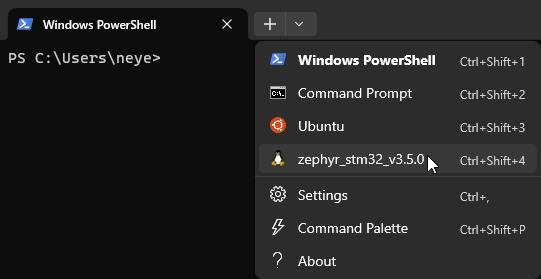
\includegraphics[width=.6\textwidth]{terminal_open_wsl_tab}
          \end{center}
        \end{infobox}
\end{itemize}

\newpage

\section{Setup with a Container Runtime}


\begin{itemize}
  \item Install the \textbf{J-Link Software and Documentation pack
          (\href{https://www.segger.com/downloads/jlink}{Download})}.
  \item Install a serial terminal like \mono{minicom}.
  \item Install a container runtime (e.g. \emph{podman} or \emph{docker}).
  \item Load the image
        \begin{lstlisting}
podman load --input @\imagename{}@.tar.gz
\end{lstlisting}
  \item Run the container
        \begin{lstlisting}
podman run --rm -it --network="host" \
  -v /path/to/project:/root/dev \
  @\imagename{}@
\end{lstlisting}
\end{itemize}

\newpage

\section{Using the Container}

\subsection{Build Sample}

Run the following inside the environment to compile the blinky sample.

\begin{lstlisting}
cd ~/zephyrproject/zephyr/samples/basic/blinky/
west build --pristine --board stm32f429i_disc1 --build-dir /tmp/build
\end{lstlisting}

\subsection{Flash Sample}

To flash from within the container the \emph{J-Link Remote Server} is used.
Start the J-Link Remote Server on the host now.

\begin{infobox}
  If the J-Link Remote Server shows an error try using a different port
  (19020 is the default).
\end{infobox}

Run the following command in a PowerShell to get the IP of the WSL network
adapter.

\begin{lstlisting}
@\cmdinwsl{}@ grep nameserver /etc/resolv.conf
\end{lstlisting}

Then run the following command to flash the board (replace the IP with the one
from above).

\begin{lstlisting}
west -v flash --runner jlink \
  --tool-opt='-ip 172.21.160.1:19020' \
  --build-dir /tmp/build
\end{lstlisting}

\begin{infobox}
  If you get a \emph{FAILED: Can not connect to J-Link via TCP/IP} error try
  adding a firewall rule that allows inbound connections on the WSL network
  adapter. To do that run the following command in an admin PowerShell.

  \begin{lstlisting}
New-NetFirewallRule -DisplayName "WSL" -Direction Inbound `
 -InterfaceAlias "vEthernet (WSL)" -Action Allow
\end{lstlisting}

  Firewall rules can also be managed by running \mono{wf.msc} in a PowerShell.
\end{infobox}

Open a serial terminal with e.g. PuTTY to see the log output:

\begin{lstlisting}
plink.exe -sercfg 115200 -serial com3
\end{lstlisting}

\newpage

\newgeometry{margin=1cm,bottom=2cm}
\fancyfoot{}

\appendix

\section{Containerfile}\label{containerfile}
\lstinputlisting[basicstyle=\ttfamily\footnotesize]{../Containerfile}

\end{document}

% Local Variables:
% TeX-output-dir: "build"
% TeX-master: t
% End:
